\documentclass[12pt, a4paper]{article}

\usepackage[hmargin=2.5cm, vmargin=2cm]{geometry}
\usepackage{amsthm, amssymb, mathtools, yhmath, graphicx}
\usepackage{fontspec, type1cm, titlesec, titling, fancyhdr, tabularx}
\usepackage{color}
\usepackage{unicode-math}
\usepackage{float}
\usepackage{subfig}
\usepackage{hhline}
\usepackage{comment}
\usepackage{siunitx}
\usepackage{csvsimple}
\usepackage{subcaption}

\usepackage[CheckSingle, CJKmath]{xeCJK}
\usepackage{CJKulem}
\usepackage{enumitem}
\usepackage{tikz}
\usepackage[siunitx]{circuitikz}
\usepackage{wrapfig}
%\setCJKmainfont[BoldFont=cwTex Q Hei]{cwTex Q Ming}
%\setCJKsansfont[BoldFont=cwTex Q Hei]{cwTex Q Ming}
%\setCJKmonofont[BoldFont=cwTex Q Hei]{cwTex Q Ming}
\setCJKmainfont[BoldFont=cwTeX Q Hei]{cwTeX Q Ming}

\def\normalsize{\fontsize{12}{18}\selectfont}
\def\large{\fontsize{14}{21}\selectfont}
\def\Large{\fontsize{16}{24}\selectfont}
\def\LARGE{\fontsize{18}{27}\selectfont}
\def\huge{\fontsize{20}{30}\selectfont}

%\titleformat{\section}{\bf\Large}{\arabic{section}}{24pt}{}
%\titleformat{\subsection}{\large}{\arabic{subsection}.}{12pt}{}
%\titlespacing*{\subsection}{0pt}{0pt}{1.5ex}

\parindent=24pt

\DeclarePairedDelimiter{\abs}{\lvert}{\rvert}
\DeclarePairedDelimiter{\norm}{\lVert}{\rVert}
\DeclarePairedDelimiter{\inpd}{\langle}{\rangle}
\DeclarePairedDelimiter{\ceil}{\lceil}{\rceil}
\DeclarePairedDelimiter{\floor}{\lfloor}{\rfloor}

\newcommand{\unit}[1]{\:(\text{#1})}
\newcommand{\df}[1]{\mathop{}\!\mathrm{d^#1}}
\newcommand{\img}{\mathrm{i}}
\newcommand{\dD}{\mathrm{d}}
\newcommand{\dI}{\,\mathrm{d}}

\title{ \bf {\Huge 電子電路實驗2:BJT FET 特性曲線量測 }\\ 實驗結報}
\author{B02901178 江誠敏}

\begin{document}

\maketitle


\section{實驗結果}
\begin{figure}[H]
\begin{center}
  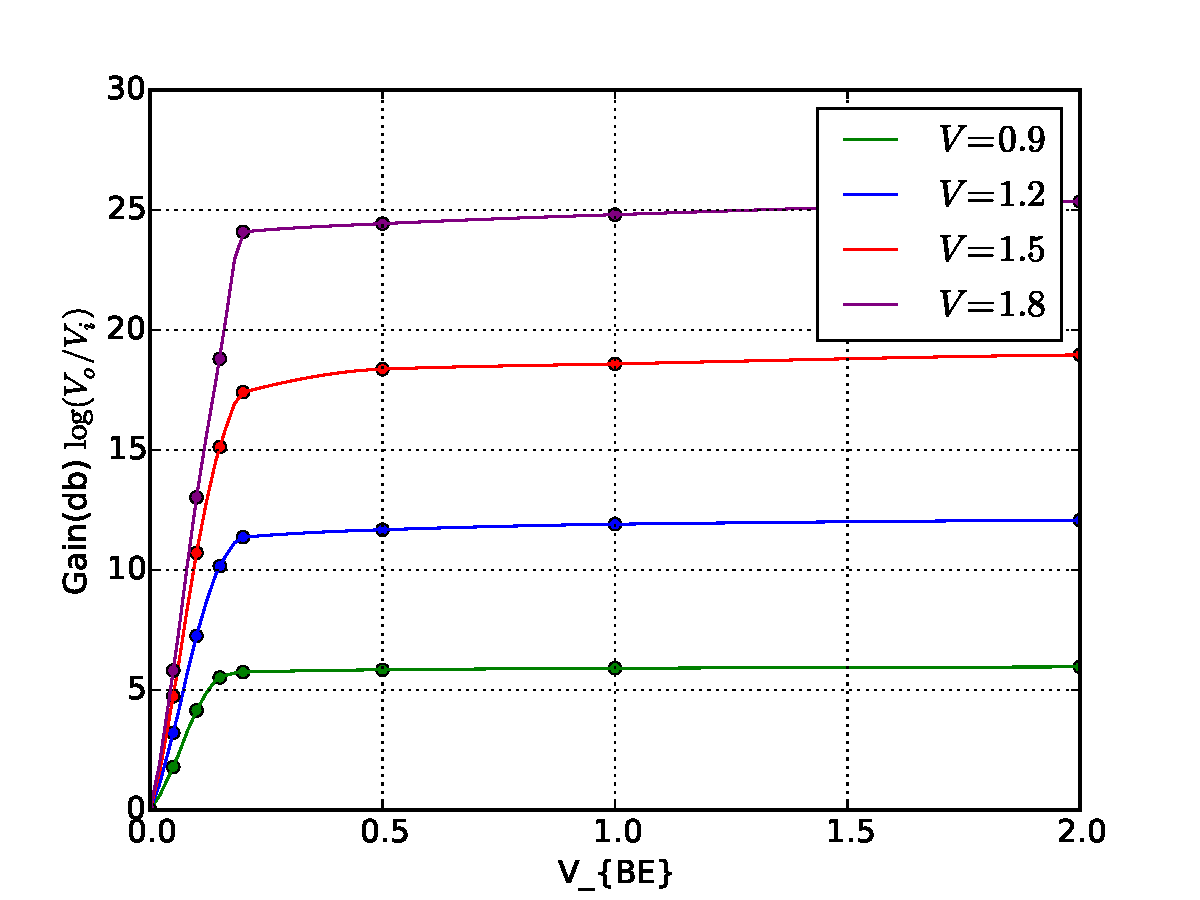
\includegraphics[width=0.75\textwidth]{fig1.pdf}
\end{center}
\caption{}
\label{fig:}
\end{figure}
~
\begin{figure}[H]
\begin{center}
  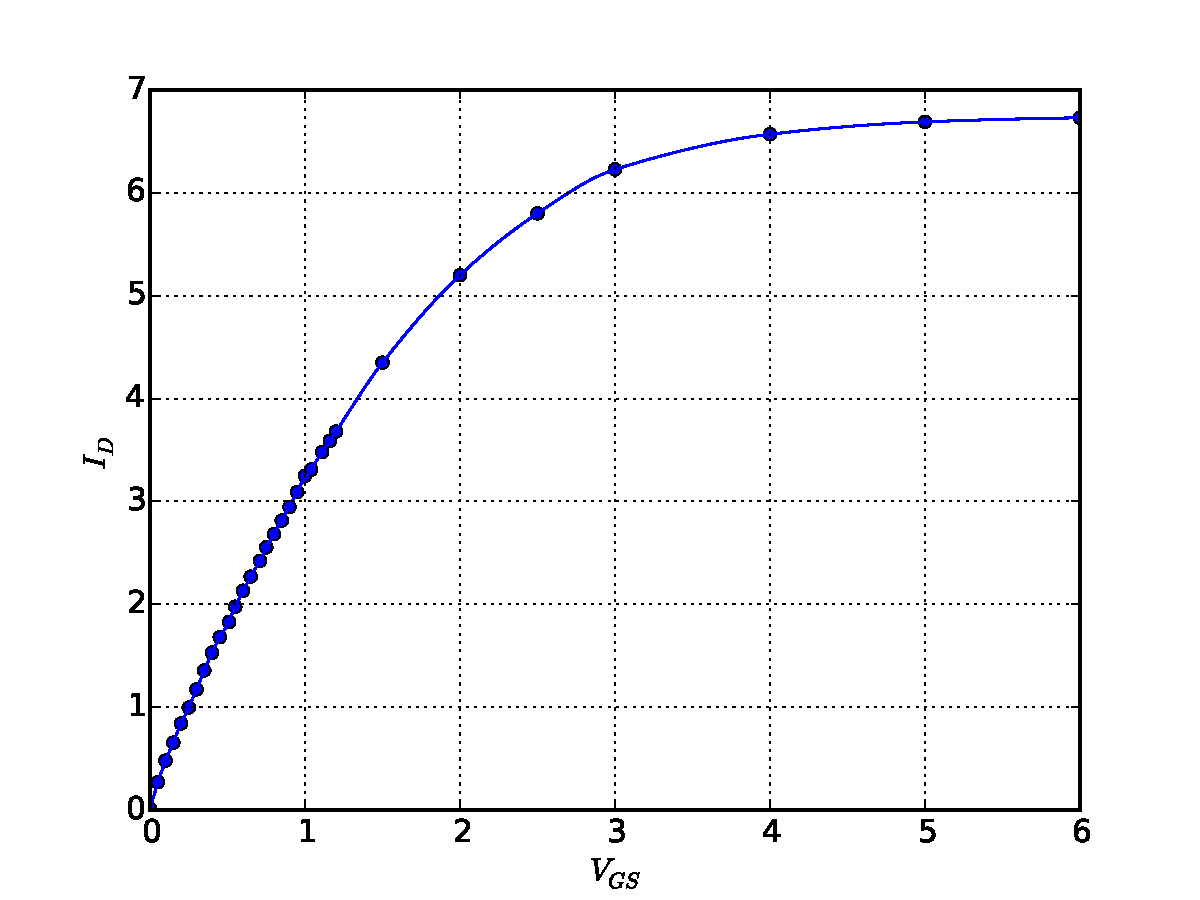
\includegraphics[width=0.75\textwidth]{fig2.pdf}
\end{center}
\caption{}
\label{fig:}
\end{figure}

\section{結報問題}

\begin{enumerate}[itemsep=20pt, topsep=10pt]

  \item {請畫出 BJT(NPN/PNP) 與 MOS(NMOS,PMOS) 元件物理結構圖。} \\[10pt]
    答:\\
    \begin{figure}[H]
      \centering
      \subfloat[][BJT npn]{
        \centering
        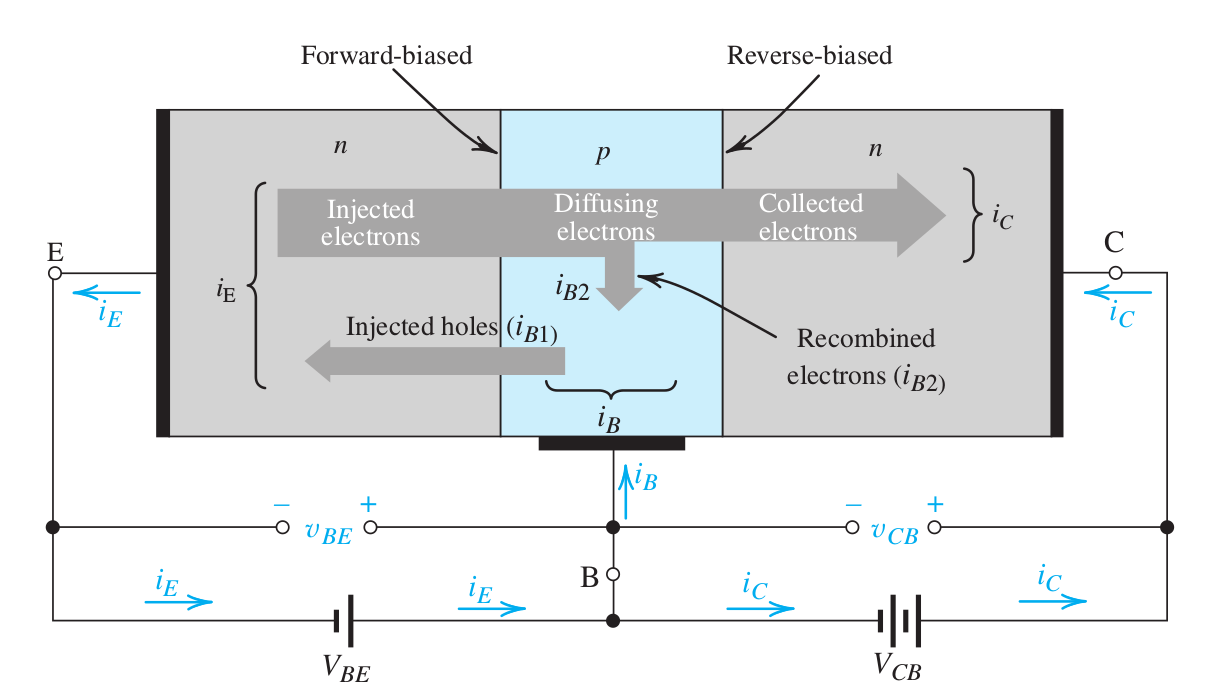
\includegraphics[width=0.75\textwidth]{npnbjt.png}
      }\\
    \end{figure}
    \begin{figure}[H]
      \ContinuedFloat
      \centering
      \subfloat[][BJT pnp]{
        \centering
        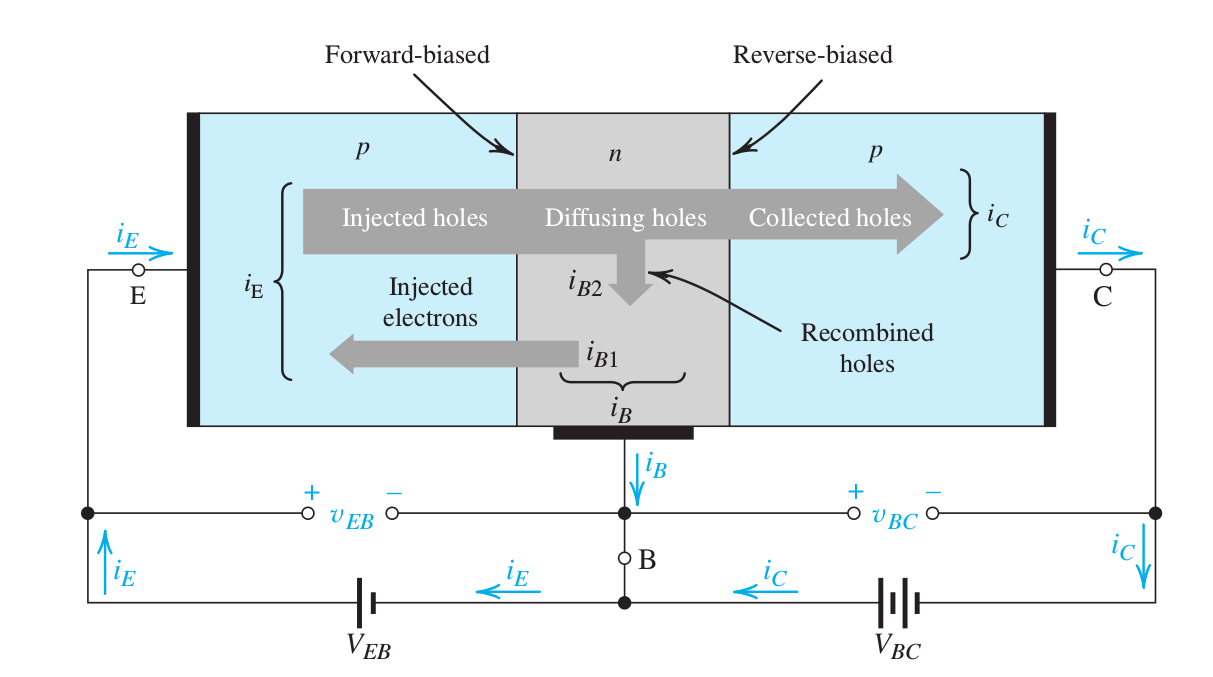
\includegraphics[width=0.78\textwidth]{pnpbjt.png}
      }\\
      \subfloat[][NMOS]{
        \centering
          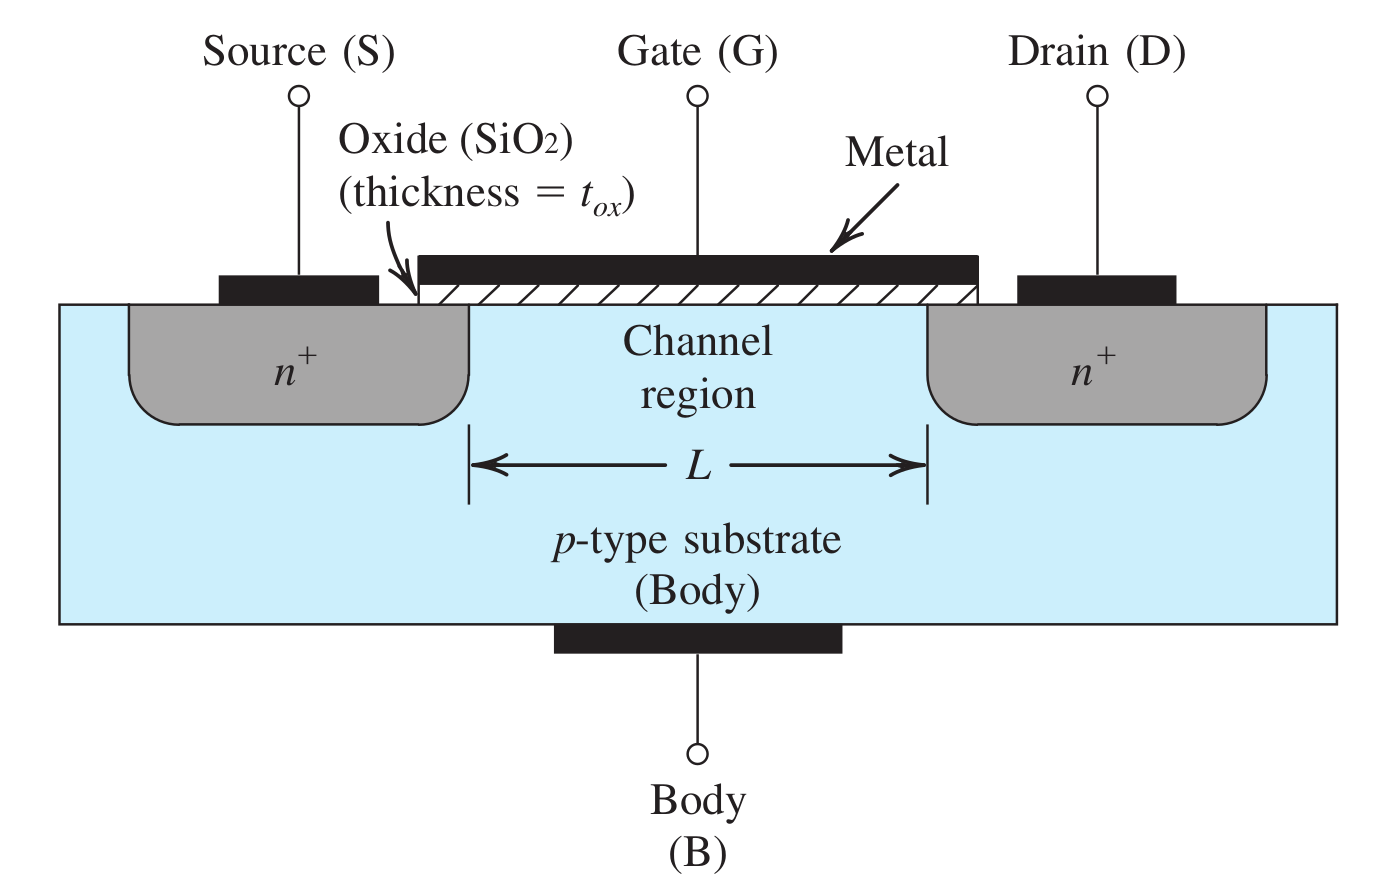
\includegraphics[width=.78\textwidth]{nmos.png}
      }\\
      \subfloat[][PMOS]{
        \centering
          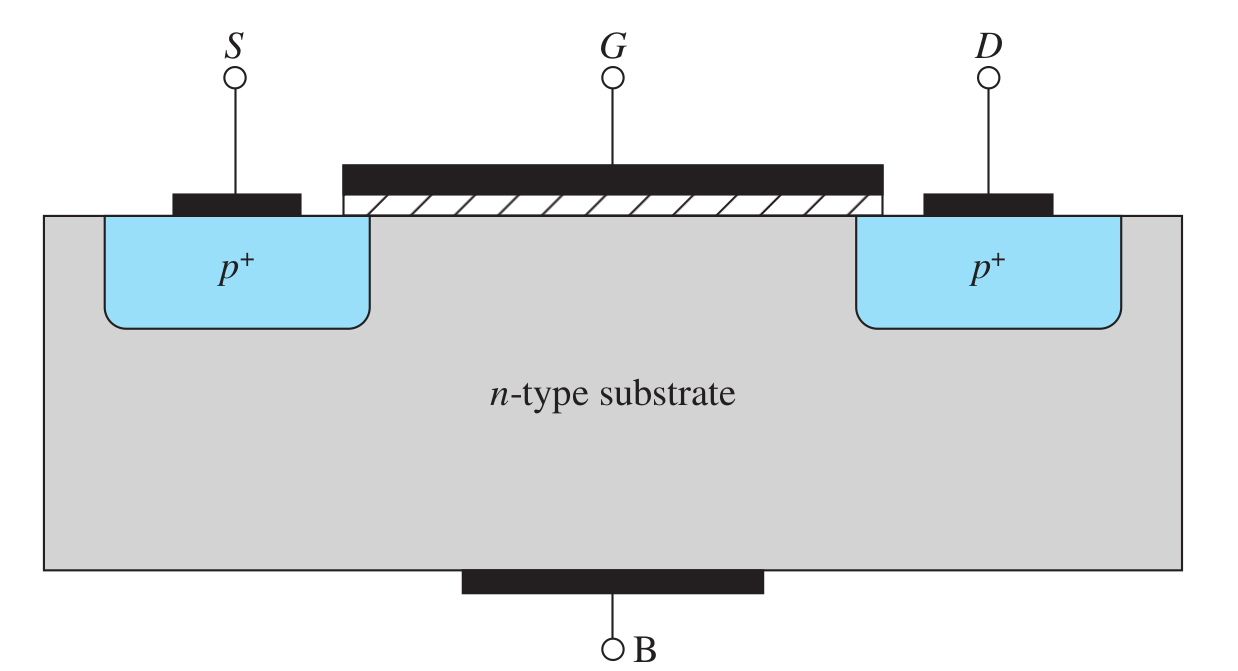
\includegraphics[width=.78\textwidth]{pmos.png}
      }
      
    \end{figure}

  \item {推導 PN diode 空乏寬度 $W$ 與障壁電壓 $V_0$。} \\[10pt]
    答:\\
    我們假設在空乏區中,電荷密度是均勻的,並且電荷密度只跟 $x$ 座標有關(因為 PN diode 是長形的)。我們可知
    \[ \nabla^2 V = \frac{\partial^2 V}{\partial x^2} = \frac{-\rho}{\epsilon_s} = \frac{q N_D}{\epsilon_s} \]
    \[ \Rightarrow V\Big\rvert_{0}^{x_n} = \frac{q N_D x^2}{2 \epsilon_s} \biggr\rvert_{0}^{x_n} =  \frac{q N_D x^2_n}{2 \epsilon_s} \]
    同樣道理,
    \[ \Rightarrow V\Big\rvert_{-x_p}^{0} = \frac{q N_A x_p^2}{2 \epsilon_s} \]
    因此
    \[
      V_0 = V\Big\rvert_{-x_p}^{x_n} = \frac{q N_D x^2_n}{2 \epsilon_s} + \frac{q N_A x_p^2}{2 \epsilon_s}
    \]
    同時因為元件是電中性,有
    \[ q A x_n N_D = q A x_p N_A \quad \Rightarrow \quad x_n N_D = x_p N_A = Z \]
    \begin{align*}
      V_0 &= \frac{qZ}{2 \epsilon_s} (x_n + x_p)  \\
      &= \frac{q Z }{2 \epsilon_s} \frac{1}{Z/N_A + Z/N_D}  (x_n + x_p)^2 \\
      &= \frac{q}{2\epsilon_s}  \frac{1}{1/N_A + 1/N_D} W^2 
    \end{align*}
    因此
    \[ W = \sqrt{ \frac{2 \epsilon}{q} \left( \frac{1}{N_A} + \frac{1}{N_D}\right)  V_0 } \]

    另外由Boltzmann distribution,可以知道電子分布的密度有下列關係
    \[
      n \propto e^{-qV /(k T)} = e^{-V/V_T} 
    \]
    因此
    \[
      N_D \approx n_n = n_p e^{- (-V_0)/V_T } = n_p e^{V_0/V_T}
    \]
    而由關係式
    \[
      n_p = \frac{n_i^2}{N_A}
    \]
    可以得出
    \[ \frac{N_D N_A}{n_i^2} = e^{V_0/V_T} \quad \Rightarrow \quad V_T \log \frac{N_D N_A}{n_i^2} = V_0 \]
    
  \item {請說明 BJT 與 MOS 的優缺點。} \\[10pt]
    答:
    \begin{itemize}
      \item BJT
        \begin{itemize}
          \item 優點:
            \begin{enumerate}[label=(\arabic*)]
              \item 輸出阻抗小。
              \item 反應較快。
              \item 放大倍率較大,有較好的Early voltage。
              \item 比較便宜。
            \end{enumerate}
          \item 缺點:
            \begin{enumerate}[label=(\arabic*)]
              \item 受溫度影響較劇烈。
              \item 消耗功率較大。
            \end{enumerate}
        \end{itemize}
      \item MOS
        \begin{itemize}
          \item 優點:
            \begin{enumerate}[label=(\arabic*)]
              \item 體積較小。
              \item 接近無限大的 Gate 端輸入阻抗。
              \item 能做為較好的開關元件。
            \end{enumerate}
          \item 缺點:
            \begin{enumerate}[label=(\arabic*)]
              \item 反應速度慢。
            \end{enumerate}
        \end{itemize}
    \end{itemize}
  \item {請說明為何 n-type 元件較常被使用。} \\[10pt]
    答:
    因為電子的 mobility 較電洞來的大,因此 n-type 元件反應速度會較
    p-type 元件快,阻抗與能量耗損也較小。
  \item {請說明 CMOS 的優缺點。} \\[10pt]
    答:
    \begin{itemize}
      \item 優點: 消耗的功率較小。
      \item 缺點: 有較大的電容效應,因此反應速度較慢。
    \end{itemize}
  \item {請說明 BiCMOS 的優缺點。} \\[10pt]
    答:
    \begin{itemize}
      \item 優點: 同時有 MOS 和 CJT 的功能。
      \item 缺點: 在製程上較為困難,因此價格昂貴。
    \end{itemize}

\end{enumerate}

\section{心得}
這次的實驗本來以為很簡單,輕輕鬆鬆做。沒想到我旁邊的同學做一做,
就覺得很奇怪,怎麼輸出的電流那麼大,於是就摸了一下 BJT 看看。沒
想到一摸,手就被燙到了,哇哇慘叫。害的我們之後做實驗戰戰兢兢,
電壓都不敢調太大。這個故事告訴我們實驗最好不要做太快,等你旁邊的
人確定可以 work 不會出事在做…
\end{document}

